\documentclass[a4paper,11pt,final]{article}
\usepackage[czech]{babel}
\usepackage[left=2cm,top=3cm,
textheight=24cm,textwidth=17cm]{geometry}
\usepackage[T1]{fontenc}
\usepackage[utf8x]{inputenc}
\usepackage{times}
\usepackage{amsmath}
\usepackage{amsthm}
\usepackage{amsfonts}
\usepackage{multirow}
\usepackage{graphicx}
\usepackage[linesnumbered, ruled, czech]{algorithm2e}
\usepackage{pdflscape}
\usepackage{hyperref}

\urlstyle{rm}
\begin{document}
	\begin{titlepage}
		\setcounter{page}{0}
		\begin{center}	
			\addtolength{\parskip}{0.6em}
			{\Huge
				\textsc{
					Vysoké učení technické v Brně}}
			
			{\huge 
				\textsc{
					Fakulta informačních technologií}}
			
			\vspace{\stretch{0.382}}
			{\LARGE
				Typografie a publikování\,--\,3. projekt
				
				\Huge Tabulky a obrázky}
			
			\vspace{\stretch{0.618}}
		\end{center}
		{\Large 
			\today \hfill Danil Domrachev (xdomra00)}
	\end{titlepage}
	
	\newpage
	\section{Úvodní strana}
	
	Název práce umístěte do zlatého řezu a nezapomeňte uvést \uv{dnešní} datum a vaše jméno a~příjmení
	
	\section{Tabulky}
	
	Pro sázení tabulek můžeme použít buď prostředí {\ttfamily tabbing} nebo prostředí {\ttfamily tabular}
	
	\subsection{Prostředí \ttfamily tabbing} 
	
	Při použití {\ttfamily tabbing} vypadá tabulka následovně:
	
	\begin{tabbing}
		Vodní melouny \quad \= Cena\quad \= Množství\kill
		\textbf{Ovoce} \> \textbf{Cena} \> \textbf{Množství}\\
		Jablka \> 25,90 \> 3\,kg\\
		Hrušky \> 27,40 \> 2,5\,kg\\
		Vodní melouny \> 35,-- \> 1\,kus
	\end{tabbing}
	
	{\raggedright
	Toto prostředí se dá také použít pro sázení algoritmů, ovšem vhodnější je použít prostředí {\ttfamily algorithm} nebo {\ttfamily algorithm2e} (viz sekce \ref{algos})}
	
	\subsection{Prostředí {\ttfamily tabular}} 	
	
	Další možností, jak vytvořit tabulku, je použít prostředí {\ttfamily tabular}. Tabulky pak budou vypadat takto\footnote{Kdyby byl problem s {\ttfamily cline}, zkuste se podívat třeba sem: \url{https://www.abclinuxu.cz/tex/poradna/show/325037}.}
	
	\catcode`\-=12
	\begin{table}[h]
		\centering
		\begin{tabular}{|c|c|c|}
			\hline
			& \multicolumn{2}{c|}{\textbf{Cena}} \\
			\cline{2-3}
			\textbf{Měna} & \textbf{nákup} & \textbf{prodej}\\
			\hline
			EUR & 24,775 & 25,943\\
			GBP & 29,394 & 30,492\\
			USD & 22,423 & 23,661\\
			\hline
	
		\end{tabular} 
		\caption{Tabulka kurzů k dnešnímu dni}
		\label{meny}
	\end{table}

	\begin{table}[h]
	\centering
	\begin{tabular}{|c|c|}
		\hline
		$A$ & $\neg A$\\
		\hline
		\textbf P & N \\
		\textbf O & O \\
		\textbf X & X \\
		\textbf N & P \\
		\hline	
	\end{tabular} 
	\begin{tabular}{|c|c|c|c|c|c|}
		\hline
		\multicolumn{2}{|c|}{\multirow{2}{*}{$A \wedge B$}} & \multicolumn{4}{c|}{$B$}\\
		\cline{3-6}
		\multicolumn{1}{|c}{ } &  & \textbf P & \textbf O & \textbf X & \textbf N \\
		\hline 	
		\multirow{4}{*}{$A$} & \textbf P & P & O & X & N \\
		\cline{2-6}
		& \textbf O & O & O & N & N \\
		\cline{2-6}
		& \textbf X & X & N & X & N \\
		\cline{2-6}
		& \textbf N & N & N & N & N \\
		\hline
	\end{tabular}
	\begin{tabular}{|c|c|c|c|c|c|}
		\hline
		\multicolumn{2}{|c|}{\multirow{2}{*}{$A \vee B$}} & \multicolumn{4}{c|}{$B$}\\
		\cline{3-6}
		\multicolumn{1}{|c}{ } &  & \textbf P & \textbf O & \textbf X & \textbf N \\
		\hline 	
		\multirow{4}{*}{$A$} & \textbf P & P & P & P & P \\
		\cline{2-6}
		& \textbf O & P & O & P & O \\
		\cline{2-6}
		& \textbf X & P & P & X & X \\
		\cline{2-6}
		& \textbf N & P & O & X & N \\
		\hline
	\end{tabular}
	\begin{tabular}{|c|c|c|c|c|c|}
		\hline
		\multicolumn{2}{|c|}{\multirow{2}{*}{$A \rightarrow B$}} & \multicolumn{4}{c|}{$B$}\\
		\cline{3-6}
		\multicolumn{1}{|c}{ } &  & \textbf P & \textbf O & \textbf X & \textbf N \\
		\hline 	
		\multirow{4}{*}{$A$} & \textbf P & P & O & X & N \\
		\cline{2-6}
		& \textbf O & P & O & P & O \\
		\cline{2-6}
		& \textbf X & P & P & X & X \\
		\cline{2-6}
		& \textbf N & P & P & P & P \\
		\hline
\end{tabular}
	\caption{Protože Kleeneho trojhodnotová logika už je \uv{zastaralá}, uvádíme si zde příklad čtuřhodnotové logiky}
	\label{logic}
\end{table}
\catcode`\-=13 	

\pagebreak



\section{Algoritmy}
\label{algos}

{\raggedright
Pokud budeme chtít vysázet algoritmus, můžeme použít prostředí {\ttfamily algorithm}\footnote{Pro nápovědu, jak zacházet s prostředím {\ttfamily algorithm}, můžene zkusit tuhle stránku: \raggedright{
\url{http://ftp.cstug.cz/pub/tex/CTAN/macros/latex/contrib/algorithms/algorithms.pdf}}} nebo {\ttfamily algorithm2e}\footnote{Pro {\ttfamily algorithm2e} zase tuhle: \url{http://ftp.cstug.cz/pub/tex/CTAN/macros/latex/contrib/algorithms/algorithms.pdf}}.
 
Příklad použití prostředí  {\ttfamily algorithm2e} viz \autoref{fastslam}}
\IncMargin{1.5em}
\begin{algorithm}[h]
	\caption{\textsc{FastSLAM}}
	\label{fastslam}
	\DontPrintSemicolon
	\SetAlgoLongEnd
	\SetAlgoNoLine
	\SetNlSty{textmormal}{}{:}
	\SetKwInOut{Input}{Input}\SetKwInOut{Output}{Output}
	\Indm\Indm
	\Input{$(X_{t-1}, u_t, z_t)$}
	\Output{$X_t$}
	\BlankLine
	\Indp\Indp
	$\overline{X_t} = X_t = 0$\;
	\For{$k = 1$ {\textnormal to} $M$}
	{
		$x^{[k]}_{t} = sample\_motion\_model(u_t,x_{t-1}^{[k]})$\;
		
		$\omega^{[k]}_{t} = measurement\_model(z_t,x^{[k]}_{t}, m_{t-1})$\;
		
		$m^{[k]}_{t} = updated\_occupancy\_grid(z_t, x^{[k]}_{t},m_{t-1}^{[k]})$\;
		$\overline{X_t} = \overline{X_t} + \langle x^{[k]}_{t}, \omega^{[k]}_{t} \rangle$
	}	
	\For{$k = 1$ {\textnormal to} $M$}
	{
		draw $i$ with probability $\approx \omega^{i}_t$\;
		add $\langle x^{[k]}_{x}, \omega^{[k]}_{t} \rangle$ to $X_t$\;
	}
	\Return{$X_t$}	

\end{algorithm}
\DecMargin{1.5em}

\section{Obrázky}

Do našich článků můžeme samozřejmě vkládat obrázky. Pokud je obrázkem fotografie, můžeme klidně použít bitmapový soubor. Pokud by to ale mělo být nějaké schéma nebo něco podobného, je dobrým zvykem takovýto obrázek vytvořit vektorově.

\begin{figure}[h]
	\centering
	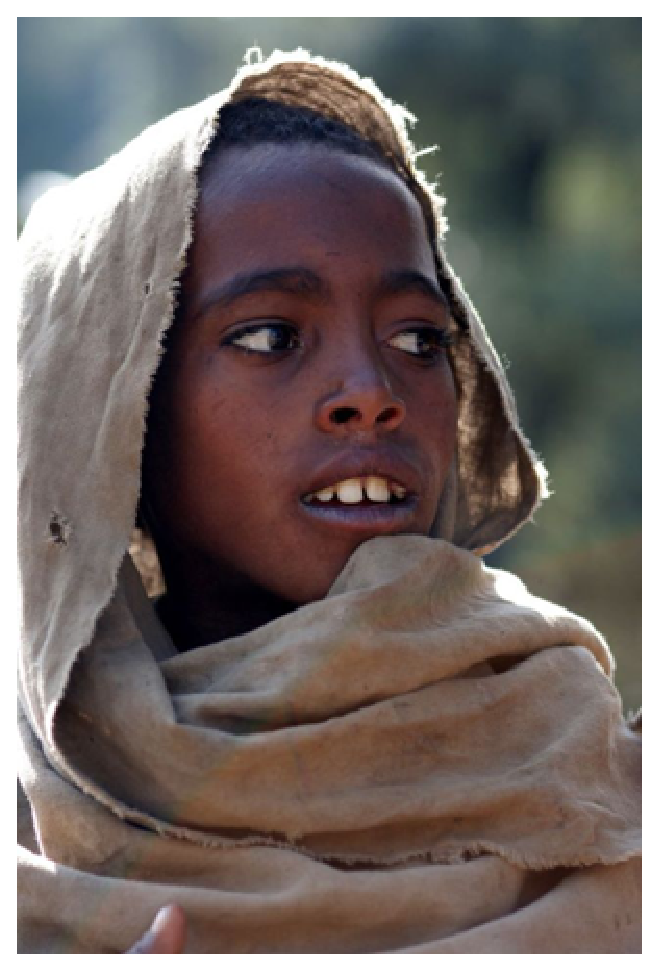
\includegraphics[scale=0.4]{etiopan}
	\reflectbox{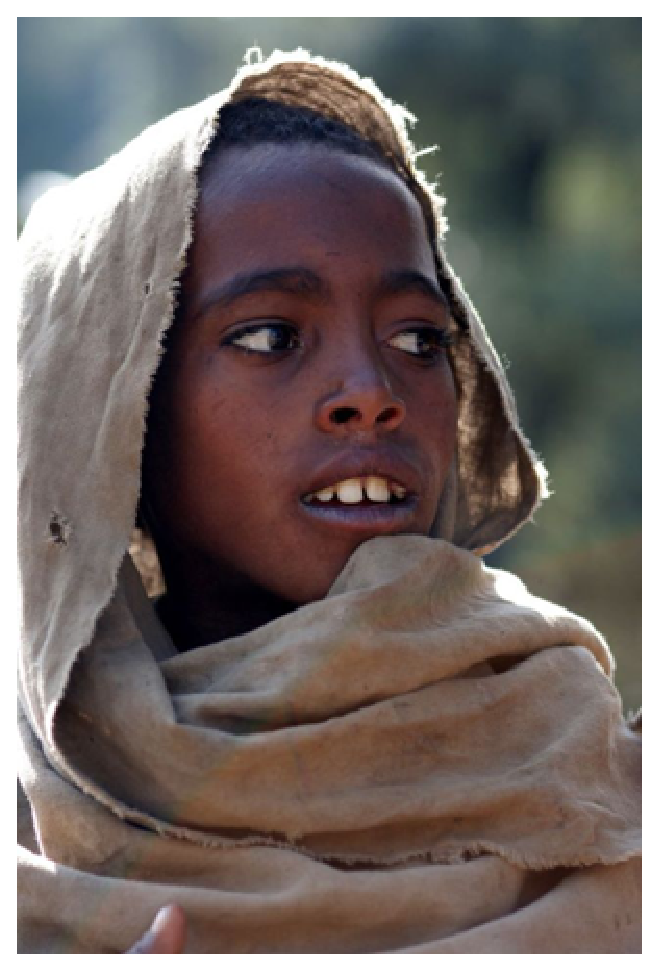
\includegraphics[scale=0.4]{etiopan}}
	\caption{Malý Etiopánek a jeho bratříček}
	\label{etiop}
\end{figure}

\newpage

Rozdíl mezi vektorovým\,\ldots

\begin{figure}[h]
	\centering
	
\includegraphics[scale=0.4]{oniisan}
	\caption{Vektorový obrázek}
	\label{vect}
\end{figure}

{\raggedright\ldots\,a bitmapovým obrázkem}

\begin{figure}[h]
	\centering
	
\includegraphics[scale=0.6]{oniisan2}
	\caption{Bitmapový obrázek}
	\label{bitm}
\end{figure}

{\raggedright se projeví například při zvětšení.}

Odkazy (nejen ty) na obrázky \ref{etiop}, \ref{vect} a \ref{bitm}, na tabulky \ref{meny} a \ref{logic} a také na algoritmus \ref{fastslam} jsou udělany pomocí křížových odkazů. Pak je ovšem potřeba zdrojový soubor přeložit dvakrát
 
Vektorové obrázky lze vytvořit i přímo v \LaTeX u, například pomocí prostředí {\ttfamily picture} 

\newpage
\begin{landscape}
	\begin{figure}[h]
		\centering
		\begin{picture}(600, 300)(0, 0)

			\linethickness{2pt}
			\put(0, 0){\line(1, 0){599}}
			\put(599, 0){\line(0, 1){299}}
			\put(0, 0){\line(0, 1){299}}
			\put(0, 299){\line(1, 0){599}}
			
			\put(540, 250){\circle{50}}
			
			\linethickness{4pt}
			\put(10, 50){\line(10, 0){580}}
			\linethickness{2pt}
			
			\put(80, 50){\line(0, 1){100}}
			\put(80, 150){\line(1, 0){120}}
			
			\put(200, 135){\line(0, 1){30}}
			\put(200, 165){\line(1, 0){130}}
			\put(330, 135){\line(0, 1){30}}
			\put(330, 140){\line(1, 0){140}}
			\put(470, 135){\line(0, 1){5}}
			
			\put(150, 135){\line(1, 0){350}}
			\put(150, 120){\line(1, 0){350}}
			\put(150, 120){\line(0, 1){15}}
			\put(500, 120){\line(0, 1){15}}
			
			\put(120, 50){\line(0, 1){50}}
			\put(120, 100){\line(1, 0){100}}
			\put(220, 100){\line(1, -1){50}}
			
			\put(150, 120){\line(1, -1){20}}
			
			\put(230, 90){\line(0, 1){25}}
			\put(230, 115){\line(1, 0){260}}
			\put(490, 75){\line(0, 1){40}}
			\put(245, 75){\line(1, 0){255}}
			\put(500, 50){\line(0, 1){25}}	

		\end{picture}

	\caption{Vektorový obrázek moderního bydlení vhodného pro 21.\,století.}
	\end{figure}
\end{landscape}

\end{document}